\section{Motivation}

This thesis, a collaboration between \href{https://www.epidemicsound.com/}{Epidemic Sound} (ES) and the \href{https://www.upf.edu/web/mtg}{Music Technology Group} (MTG) at Universitat Pompeu Fabra (UPF), has been driven by personal, academic, and industrial motivations. ES, a Swedish company, curates a vast global library of over 40,000 royalty-free music tracks and 90,000+ sound effects. Based in Barcelona, MTG specializes in innovative sound and music technologies, such as information retrieval, digital signal processing, interactive music systems, and computational musicology.

The collaboration aims to deepen our understanding of music's fundamental structures, which could enhance ES's technical offerings and further advancements in music information retrieval (MIR) research.

As a musician, enthusiast, and scholar, my passion for music has driven me to investigate the foundational elements of musical composition, various creation techniques, and their intricate relationships. I am dedicated to extracting valuable information embedded within music across all domains, with a particular focus on audio and symbolic. Musicians who endeavor to bridge the gap and uncover musical truths within the tonal paradigm, such as Heinrich Schenker \cite{Komar1959SchenkersStructure}, or those who challenge it, like Arnold Schoenberg \cite{Samson1974SchoenbergsMusic}, George Russell \cite{LydianRussell}, and Ernst Levy \cite{LevyAHarmony}, have been a continual source of inspiration. They aim to identify abstract concepts that reinforce or disrupt the tonal foundation, advancing the tonal landscape and providing a solid base for musicians' growth, development, and understanding of tonal and atonal paradigms.

Advancements in AI research, building on the theoretical groundwork laid by pioneers such as Alan Turing and Claude Shannon, have led to significant breakthroughs \cite{Vaswani2017AttentionNeed}. With AI being applied broadly in popular products \cite{OpenAI2023GPT-4Report}, researchers and corporations alike must stay abreast of this rapidly evolving field. The emergence of self-supervised models capable of learning embedding spaces to retrieve musical content from audio signals presents new opportunities. These models, which autonomously extract high-level semantic information from raw audio data, can potentially transform multiple aspects of the music industry. Industrially, these embedding spaces can be used to devise innovative products, enhance user experiences for content creators, and stimulate innovation and collaboration across the industry.

Traditionally, MIR research has focused primarily on technical aspects, perhaps overlooking relevant areas such as perception, cognition, music theory, musicology, aural skills, and high-level perceptual concepts. Purely mathematical approaches may not accurately represent human music perception and could miss subtle variations in timing or harmonic relationships essential to the musical experience. Therefore, MIR research should strive for a balanced approach, recognizing the interdisciplinary nature of music and the importance of areas beyond digital signal processing.

%%%%%%%%%%%%%%%%%%

\begin{figure}[ht]
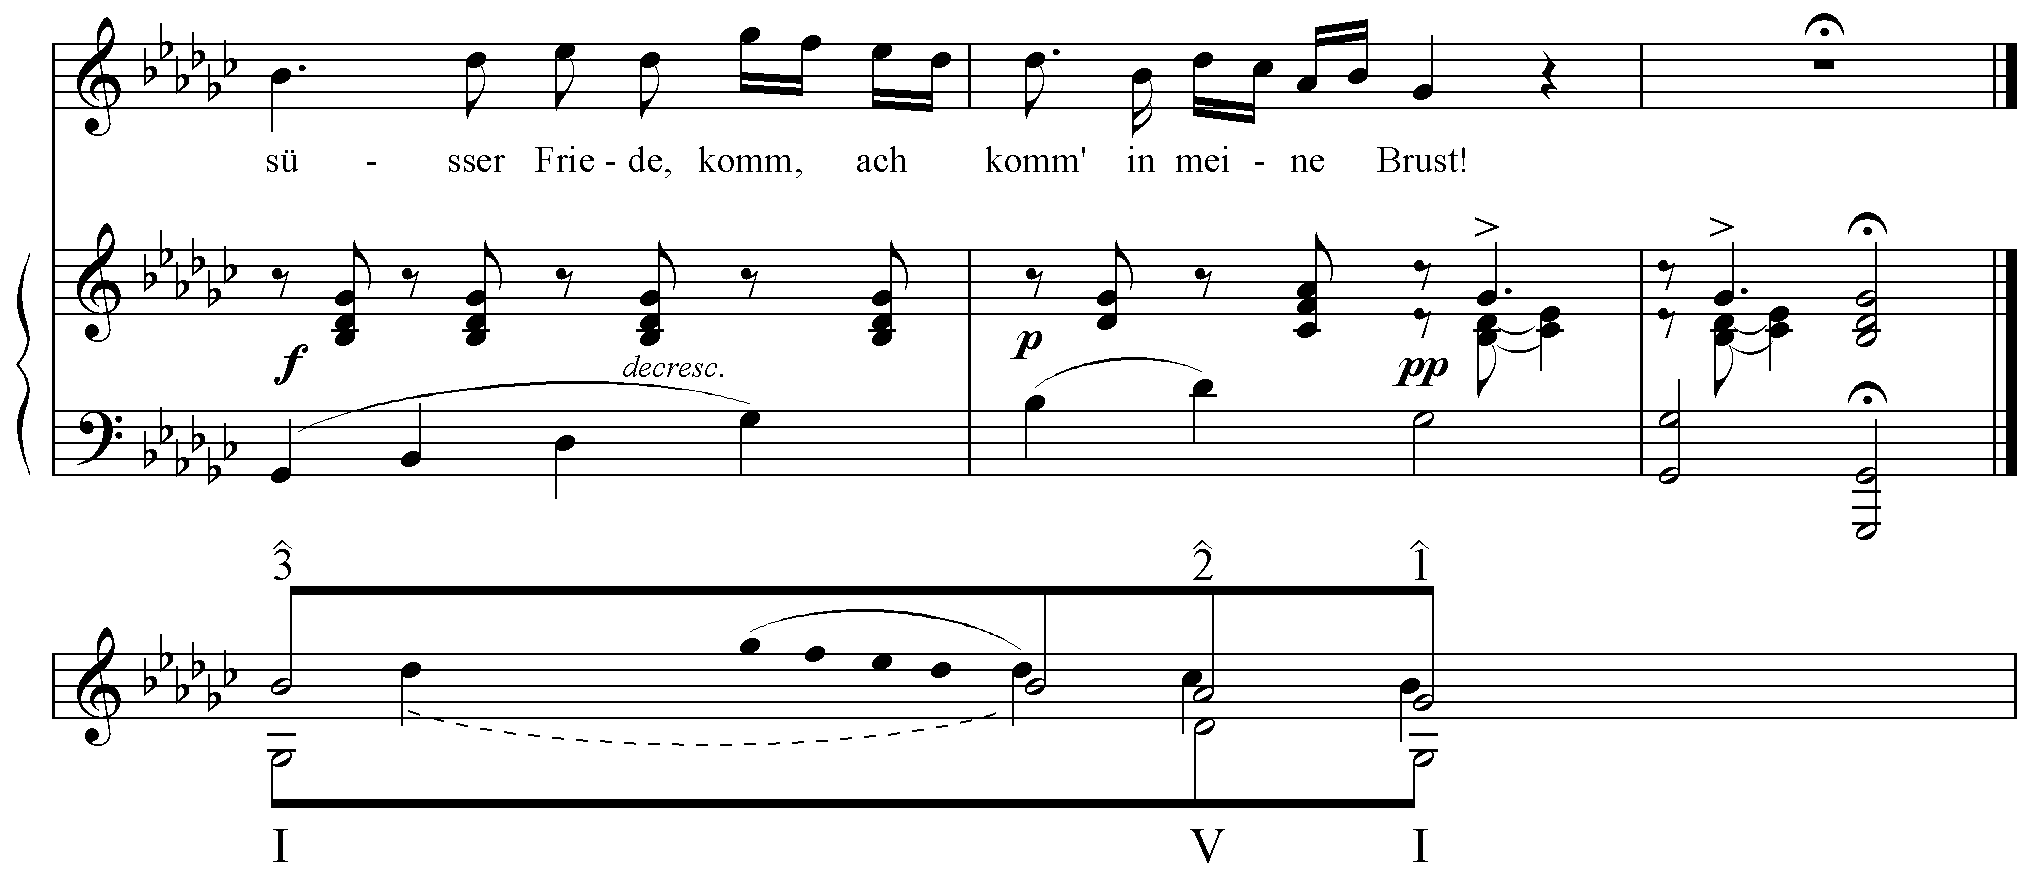
\includegraphics[clip,width=\columnwidth]{figures/schenkerian analysis/SchubertOp4no3.png}% 
\caption[Excerpt of \textit{Wandrers Nachtlied, Op. 4, D. 224} by Franz Schubert.]{\small{Small excerpt of \textit{Wandrers Nachtlied, Op. 4, D. 224} by Franz Schubert. Passage's original score, the schenkerian unfolding of the melody, the chord degrees analysis, and their tonal function.}}
\label{fig:Wandrers Nachtlied, Op. 4, D. 224}
\end{figure}